\documentclass{article}
\usepackage{amsfonts}
\usepackage{amsthm}
\usepackage{amssymb}
\usepackage{amsmath}
\usepackage{graphicx}
\usepackage{subcaption}
\usepackage[shortlabels]{enumitem}
\usepackage{xcolor}
\usepackage{tikz}

\newcommand{\new}[1]{
    \vspace{2mm}
    \noindent
    \textbf{
    \underline{#1}}
}

\def\calO{{\mathcal{O}}}
\def\th{{\theta}}
\def\_{{\hspace{1mm}}}
\def\<{{\langle}}
\def\>{{\rangle}}


\newcounter{problemcnt}
\setcounter{problemcnt}{0}

\newcommand{\Problem}{{
    \vspace{5mm}
    \stepcounter{problemcnt}
    \noindent
    \arabic{problemcnt}. 
}
}

\newcommand{\nProblem}[1]{
    \vspace{5mm}
    \noindent
    \setcounter{problemcnt}{#1}
    \arabic{problemcnt}. 
}


\newcommand{\Proof}{{
    \vspace{2mm}
    \noindent
    \textbf{
    \underline{Proof}}
}
}

\newcommand{\textOr}{
    {
        \hspace{5mm}
        \textrm{or}
        \hspace{5mm}
    }
}

\newcommand{\textAnd}{
    {
        \hspace{5mm}
        \textrm{and}
        \hspace{5mm}
    }
}

\newcommand{\m}{
    \cdot
}

\newcommand{\Pt}[1]{
    $P_{#1}$
}

\newcommand{\Szpt}[1]{
    $|P_{#1}|$
}

\newcommand{\bbinom}[2]{
    \bigg(\binom{#1}{#2}\bigg)
}



\begin{document}
\begin{center}
\LARGE
Combinatorics HW4

\Large
Daniel Son
\end{center}


Section 4.6: 36, 37, 43, 50

Section 5.7: 3, 4, 7, 9, 15, 23, 24


\new{Additional Problem 1.}
 Draw the Hasse diagram for the divides rela-
tion on the positive divisors of 30. Then explain in your own words the
relationship between that diagram, and the diagram in Figure 4.7 from
the textbook.

\new{Solution}

\begin{center}
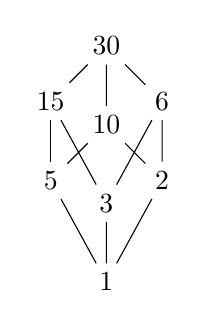
\begin{tikzpicture}
    \node(top) {$30$};
    \node(15)[below left of=top] {$15$};
    \node(10)[below of=top]{$10$};
    \node(6)[below right of=top]{$6$};
    \node(2)[below of=6] {$2$};
    \node(3)[below of=10] {$3$};
    \node(5)[below of=15]{$5$};
    \node(1)[below of=3]{$1$};
    \draw (top) -- (15) -- (3) -- (1) -- (2) -- (6) -- (top);
    \draw (15) -- (5);
    \draw (top) -- (10) -- (5) -- (1);
    \draw (3) -- (6);
    \draw (2) -- (10);
\end{tikzpicture}
\end{center}

The Hasse diagram of the divisors of 30 are isomorphic to the 
Hasse diagram of the subsets of $\{1, 2, 3\}$. We can describe the 
isomorphism as follows. Let define function $f$ to as $f(1) = 2, 
f(2) = 3, f(3) = 5$. The isomorphism $\phi$ that maps subsets 
to numbers is
\[
    \phi(S) = \prod_{k \in S} f(k) 
\]
where $S \subseteq \{1,2, 3\}$. For example, 
$\phi(\{1, 3\}) = f(1)\m f(3) = 2\times 5 = 10$. By the 
fundamental theorem of arithmetic, it is easy to see that 
each divisor correspond to a unique subset via the inverse of 
$\phi$. \hfill \qed

\new{Sec4.6Q36} 
Let X be a set of n elements. How many different relations on X are there? How 
many of these relations are reflexive? Symmetric? Antisymmetric? Reflexive 
and symmetric? Reflexive and anti-symmetric?

\new{Solution}

We distinguish any ordered pairs of two integers into distinct 
and nondistinct pairs. The former refers to the pairs 
which have distinct entries. That is $(a, b)$ where $a \neq b$. 
The latter refers to $(a, a)$. 

Relations can be considered as a set of ordered pairs. If the 
relation is symmetric, the choice of a nondistinct pair of the 
relation forces the relation to include the corresponding pair. 
That is, if $(a, b) \in R$ for where $a \neq b$, then $(b, a) \in R$. 
The choice of nondistinct pairs does not affect the symmetry of 
the relation. For a relation to be reflexive, it must include 
all the nondistinct pairs. For a relation to be antisymmetric 
it must not include any of the nondistinct pairs. 


From the observations made above, we construct relations that satisfy 
the given conditions. If the relation is defined from the cannonical 
set $[n]$ to $[n]$, there exists n nondistinct pairs and $\binom{n}{2}$
couples of distinct pairs. 

It is trivial that there exists $\boxed{2^{n^2}}$ relations overall. 

To construct all the symmetric relations, we either choose or leave 
each nondistinct pair or a distinct couple of pairs. There 
are a total of $n + \binom{n}{2}$ such objects. Thus, the 
number of symmetric relations are $\boxed{2^{n(n+1)/2}}$. 

As for the reflexive relations, we choose all the nondistinct 
pairs and choose or leave the distinct pairs. There are $n(n+1)$ 
distinct pairs so we conclude that there are $\boxed{2^{n(n-1)}}$ 
reflexive relations. 

For antisymmetric relations, we can either choose or leave 
all the nondistinct pairs. For the distinct pair couples, we 
are allowed to choose one of the two pairs, or include both of 
them from the relation. Thus, there are three possible choices 
for each distinct couple. We count $\boxed{3^{\binom{n}{2}}2^n}$. 

For reflexive and symmetric relations, we choose or 
leave the distinct couples and choose all the nondistinct pairs. There 
are $\boxed{2^{n(n-1)/2}}$ such relations. 

For reflexive and antisymmetric relations, we choose all 
the nondistinct pairs and choose between the three options 
for each distinct couple. We count $\boxed{3^{\binom{n}{2}}}$.




\new{Sec4.6Q37} Let $R', R''$ be partial orders on a set $X$. 
Define the intersection $R$ such that $xRy \leftrightarrow (xR'y) \wedge 
(xR''y)$. Prove that $R$ is a partial order. 

\proof
We demonstrate symmetry, reflexivity, and transitivity of the relation 
$R$. For $R', R''$ are both partial orders, they must be reflexive. 
Hence, $xR'x$ and $xR''x$ for any $x \in X$. By the definition of 
the intersect $R$, $xRx$. $R$ is reflexive.

To demonstrate symmetry, assume $xRy$. We deduce $xR'y$ and $xR''y$ 
from definition. $R'$ and $R''$ are symmetric, so $yR'x$ and $yR''x$. 
Thus, $yRx$ and $R$ is symmetric. 

By the same logic, we demonstrate transitivity. Assume $xRy$ and $yRz$. 
$xR'y$ and $yR'z$ from the definition of $R$ and we infer $xR'z$ from 
the transitivity of $R'$. Likewise, $xR''z$. Thus, $xRz$ which concludes 
the proof. \hfill \qed


\new{Sec4.6Q43} Let $X = {a, b, c, d, e, f}$ and let the relation $R$ on X be defined by $aRb, b R c, 
c R d, aRe, e R f, f R d$. Verify that R is the cover relation of a partially ordered 
set, and determine all the linear extensions of this partial order. 

\new{Solution}
Drawing a Hasse diagram, we identify that element $a$ 
is maximum and $d$ the minimum. All elements are connected
either upwards or downwards of $a$ and $d$. By transitivity, 
we infer all the orders, and set $xRx$ for all $x \in X$. 

As for the number of all linear extensions, we 
will count all the linear arrangement of the elements. 
Arrange the elements from the smallest to largest
The position of $d, a$ are fixed to be in the beginning 
and in the end of the queue. Any arrangement 
where $c$ comes before $b$ and $f$ comes before $e$ 
will work. Observe that by reseving the positions of 
$b, c$, a linear order is created. There are $\boxed{\binom{4}{2} = 6}$ 
ways to do this. 


\new{Sec4.6Q50}
Consider the partially ordered set of subsets of the set $X = \{a, b, c\}$ of 
three elements. How many linear extensions are there? 

\new{Solution}

Again, refer to the Hasse diagram from the book. We fix the 
entire set and the emptyset to be the maximum and the minimum of the linear 
order. Considering arranging the 8 subsets in a line, we have 
deduced the necessary position of the two elements. 

The nonempty proper subsets occupy the six remaining slots. 
We first determine the order of the three elements $\{a\}, \{b\}, \{c\}$. 
Afterwards, we insert the subsets with two elements in between to 
come up with a valid ordering. Notice that from the permutation 
$(a, b, c)$ (abusing notation so that $a = \{a\}$ and so on), the 
subsets $\{a, b\}, \{a, c\}$ must come before $\{a\}$. The set $\{b, c\}$
can either come before $\{b\}$ or $\{a\}$. For the former case, 
the three subsets of size 2 can be arranged in any of the six possible 
orderings amongst them. For the latter case,  $\{a, b\}, \{a, c\}$ 
has two possible arrangements. By the principle of addition and 
multiplication, we deduce that the total number of linear extensions 
are 
\[
    6\m(2+6) = \boxed{48}
\]

\new{Sec5.7q3}
Compute the first few diagonal sums of the Pascal's triangle. 
Determine the relationship between them. 

\new{Solution}

The nth diagonal can be considely written as the following sum. 
\[
    a_n := \sum_{i = 0} ^ {n-i\geq i} 
    \binom{n - i}{i}
\]
Where $n  = 0, 1, 2, ...$. 

The following python code generates the diagonal sum. 

\begin{verbatim}
def P(n, k):
    ans = 1
    for i in range(k):
        ans = ans * (n-i)
    return ans

def C(n, k):
    return P(n, k)/P(k, k)

def nthDiag(N):
    i = 0
    ans = 0
    while (N - i >= i):
        ans = ans + C(N - i, i)
        i = i + 1
        
    return ans
\end{verbatim}

According to python, the first few of the sums are
\[
    1, 1, 2, 3, 5, 8, 13, 21, 34, 55
\]

and we recognize that this is the fibbonacci sqeuence. 
That is, denoting the nth diagnoal sum $a_n$, 
\[
    a_{n+2} = a_{n+1}+a_{n}
\]

%prove if time allows

\new{Sec5.7q4}
Expand the following two products by the binomial theorem. 


\newcommand{\term}[2]{
    x^{#1}y^{#2}
}


\new{Solution}

\[
    (x + y)^5 = 
    \sum_{i = 0}^{i = 5} \binom{5}{i} \term{i}{5 - i}
    = y^5 + 5 x y^4 + 10 x^2 y^3 + 10 x^3 y^2 + 5 x^4 y + x^5
\]

\[
    (x + y)^6 = 
    \sum_{i = 0}^{i = 6} \binom{6}{i} \term{i}{6 - i}
    = y^6 + 6 x y^5 + 15 x^2 y^4 + 20 x^3 y^3 + 15 x^4 y^2 + 6 x^5 y + x^6
\]

\new{Sec5.7q7}
Prove that the weighted sum of the binomials by the geometric 
series is in the form of $(r+1)^k$. 

\new{Solution}
We start with considering a specific sum. Write 
\[
    \sum_{i = 0}^{i = n} \binom{n}{i} 2^i 
    = 
    \sum_{i = 0}^{i = n} \binom{n}{i} 2^i 1^{n - i} 
\]
By plugging in $(x, y) = (2, 1)$ to the binomial theorem, 
we recognize that the sum is exactly $3^n$. 
\[
    \sum_{i = 0}^{i = n} \binom{n}{i} x^iy^{n-i} = (x+y)^n
    \textAnd 
    \sum_{i = 0}^{i = n} \binom{n}{i} 2^i 1^{n - i} = (2+1)^n = 3^n
\]

Likewise, for the sum 
\[
    \sum_{i = 0}^{i = n} \binom{n}{i} r^i 
\]
plug in $(x, y) = (r, 1)$ to show that the sum is $(r + 1)^n$
\hfill \qed

\new{Sec5.7q9}
Evaluate the sum 
\[
    \sum_{i = 0}^{i = n} (-1)^i\binom{n}{i} 10^k
\]
\new{Solution}
The sum equals 
\[
    \sum_{i = 0}^{i = n} \binom{n}{i} (-10)^k 1^{n - k}
    = (-10 + 1)^n = \boxed{(-9)^n}
\]


\new{Sec5.7q15}
Prove the equality for every integer $n > 1$. 

\[
    \binom{n}{1} - 2\binom{n}{2} + \cdots + (-1)^{n-1} n \binom{n}{n} = 0  
\]

\proof 
We prove the identity by differentiating the binomial identity. 
For any positive integer $n$, 
\[
    (1-x)^n = 
    \sum_{i = 0}^{i = n} \binom{n}{i} (-x)^i
    = 1 + \sum_{i = 1}^{i = n} \binom{n}{i} {-x}^i
\]

Take the derivative with respect to $x$ both sides. 
\[
    \frac{d}{dx}(1-x)^{n}
     =  \sum_{i = 1}^{i = n} \binom{n}{i} (-1)^i \frac{d}{dx}{x}^{i}
\]

\[
    n(1-x)^{n-1} = \sum_{i = 1}^{i = n} \binom{n}{i} (-1)^i i{x}^{i - 1}
\]
Set $x = 1$ and multiply $-1$ both sides. 
\[
    0\m(-1) = \sum_{i = 1}^{i = n}(-1)^{i + 1} i \binom{n}{i} 
    =     \binom{n}{1} - 2\binom{n}{2} + \cdots + (-1)^{n-1} n \binom{n}{n} 
\]
\hfill \qed
\end{document}